\section{JOGOS}
%{{{

Segundo \autocite{indieGamesLemes} jogo digital constitui-se em uma
atividade lúdica composta por uma série de ações e decisões,
limitada por regras e pelo universo do game, que resultam em uma
condição final.

Apesar da definição clara, uma taxonomia dos jogos não é tarefa
trivial. Pela diversidade em itens e gêneros e a vasta quantidade de
dimensões que os vídeo games se encontram, uma categorização dos
jogos contemporâneos é extremamente difícil de desenvolver (muitos
já tentaram) \autocite[pp. 60]{gamebenefits}.

Para corroborar com essa complexidade \cite{gamebenefits} afirmam que
a natureza dos jogos tem mudado drasticamente na última década, se
tornando cada vez mais complexos, diversos, realísticos e sociais em
sua natureza.

Com as inovações nas tecnologias relacionadas ao HTML novas
possibilidades e gêneros de jogos podem ser explorados na WEB. Sendo
que cada gênero acompanha um conjunto de desafios específicos.
Jogos de FPS (tiro em primeira pessoa) requerem menor latência de
rede, já jogos de RPG podem requerer vastas quantidades de cache
\autocite{html5mostwanted}.

A inerente complexidade dos jogos e sua vasta utilização pelos mais
diversos públicos os tornam tópico de interesse para pesquisas.
Apesar de a quantidade de estudos sobre os males dos jogos ser
muito maior do que os estudos sobre seus benefícios, a quantidade de
benefícios já correlacionados aos jogos é grande.

\autocite{gamebenefits} demostra que vídeo games melhoram as funções
cognitivas, as capacidades criativas, e motivam uma visão positiva
diante a falha. Também segundo \autocite{gamebenefits} postura positiva
em relação a falha correlaciona-se com melhor performance acadêmica.

Benefícios em habilidades práticas também são observados em
usuários de jogos. Jogadores de jogos de tiro demonstram maior
alocação de atenção, maior resolução espacial no processamento
visual e melhor habilidades de rotação \autocite{gamebenefits}.

Estes aspectos positivos muitas vezes não recebem a atenção devida.
Habilidades espaciais derivadas de jogar jogos de tiro comercialmente
disponíveis são comparáveis aos efeitos de um curso universitário
que busca melhorar as mesmas habilidades \autocite{gamebenefits}. Estas
habilidades derivadas dos jogos são centrais para muitas áreas de
interesse humano, \cite{gamebenefits} afirmam que habilidades espaciais
estão diretamente relacionadas com o sucesso em ciência, tecnologia,
engenharia e matemática.

Outra outro ponto importar dos jogos é seu aspecto social. Apesar de a
mídia ter criado uma perspectiva negativa sobre jogos, especialmente
os violentos, a realidade é mais complexa do que se pensa. Jogadores
de jogos violentos, cuja jogabilidade encoraje a cooperatividade, são
mais prováveis de exibir comportamento altruísta fora do contexto dos
jogos, do que jogadores de jogos não violentos \autocite{gamebenefits}.

\cite{html5mostwanted} ressalta a importância do planejamento antes do
desenvolvimento de jogos. Ao criar jogos deve-se planejar o que se
pretende atingir e como chegar lá antes de se escrever qualquer
código.

\subsection{MECÂNICA}

A mecânica é composta pelas regras do jogo. Quais as ações
disponíveis aos usuários, é fortemente influenciada pela categoria do
jogo em questão. Dedicar-se na elaboração de uma mecânica é tarefa
quintessencial para a construção de um jogo de sucesso.

\autocite{html5mostwanted} afirma que se os gráficos e áudio são
espetaculares mas a jogabilidade é chata o jogador vai parar de jogar.
A substância do jogo é sua mecânica, então não invista muito em
visual ao menos que isso desempenhe um papel essencial no jogo.

A elaboração da mecânica em jogos desenvolvidos profissionalmente
pode ser integrada dentro de um processo de engenharia de software
\footnote{O sumário também conta com um resumo sobre metodologias de
desenvolvimento de software contextualizada para a criação jogos}.
Os desenvolvedores tem que evitar fazer o jogo para eles mesmos.
Falta de crítica  antes do desenvolvimento também tende a gerar criações ruins.
Bons jogos são aqueles que ao menos  suprem as expectativas dos usuário.
\cite{indieGamesLemes} aponta alguns fatores procurados pelos usuários
de jogos: Desafio, socializar, experiência solitária, respeito e
fantasia.

\section{Laço do jogo}

Os jogos são dirigidos por um laço que executa uma série de tarefas
a cada frame, construindo a ilusão de um mundo animado \autocite[pp.
31]{gwt}. O laço do jogo (\textit{game loop}) é peça central em
praticamente qualquer jogo eletrônico. A cada iteração do jogo
o laço é executado e o processamento de entrada de usuário e
computações correlacionadas são executadas.

Para escrever o laço é possível utilizar as funções do JavaScript
\textit{window.settimeout}. Não obstante, a forma mais recomendada é
utilizar o \textit{window.requestAnimationFrame} reduz ou completamente
para a execução do laço enquanto o usuário está em outra aba.
Isso reduz o consumo de bateria, uma característica importante para
dispositivos móveis.

\section{JOGOS MULTIPLATAFORMA}
\begin{draft}
Jogos para múltiplas plataformas trazem um novo conjunto de desafios
para produtores de jogos. Um destes desafios é fornecer feedback
suficiente para o jogador pois muitas vezes o dispositivo é limitado em
proporções, som, tela. Outro desafio é suportar os vários ecossistemas
de software com tecnologias diferenciadas e versões de software
divergentes.

%A interface tem que ser o mais intuitiva o possível. No caso de
%dispositivos móveis, quanto menos gestos necessários melhor. Tornar
%previsível causa e efeito é uma boa característica para esta classe de jogos.

\cite{html5mostwanted} afirma que: o estágio mais complicado e crucial
do desenvolvimento de jogo é a escolha das tecnologias utilizadas.
Designers de jogos tem as seguintes possibilidades quando em face
de desenvolver um jogo multiplataforma: criar um jogo web, um jogo
híbrido, ou nativo. As opções serão descritas abaixo.

\subsection{JOGOS WEB}

%Este tipo de jogo é o que será abordado neste trabalho. 

Um jogo web é um jogo que utiliza o HTML e ferramentas correlacionadas
para sua construção.

O objetivo primário da WEB nunca foi o desenvolvimento de
jogos, mas as novas versões do HTML estão provendo funcionalidades
que permitem a criação de conteúdo interativo, incluindo jogos.

Por muito tempo os títulos famosos de jogos da web residiam em jogos
como \textit{Traviam}, desprovidos de animações, compostos basicamente
por formulários, imagens e textos. Não obstante, publicar jogos
baseados em texto é uma atividade cada vez mais rara, podendo-se
concluir que interface gráfica se tornou uma funcionalidade mandatória
\autocite{browserGamesTechnologyAndFuture}.

Durante esse período o interesse em jogos WEB residia principalmente
nas de casualidade, flexibilidade, e o fator social dos jogos.
Características essas que descrevem peculiaridades WEB no geral,
fatores que não são exclusivos de jogos.

Mais recentemente é que a WEB começou a ser vista como de fato um
ambiente com interatividade para criação de jogos dos mais variados
gêneros. Jogos como Angry Birds, Crush Candy Saga, entre outros
títulos expandiram os conceitos do que é possível se fazer utilizando
as ferramentas da WEB. Segundo \cite[pp. 28]{gwt} um bom exemplo
que tem alcançado bastante sucesso entre o público são os jogos
adicionados no logotipo do Google, chamados doodles.

Quando comparados a outras abordagens de criar jogos, jogos da WEB
contém vários aspectos positivos. Talvez o mais reconhecível
é o fato de com uma única base de código poder suprir uma gama
praticamente inesgotável de dispositivos. Comparável a base de
clientes está a quantidade de desenvolvedores WEB, os quais podem
reaproveitar grande parcela do conhecimento adquirido através do
desenvolvimento de páginas WEB na criação de jogos. O custo do
desenvolvimento de jogos também é reduzido devido a inexistência de
duplicação de código. Jogos WEB não requerem atualizações manuais.
Sua distribuição é superior ao estilo convencional de aplicações
desktop \autocite{browserGamesTechnologyAndFuture}. Por serem
criados à partir das tecnologias da WEB se beneficia de uma arquitetura
construída para um ambiente social, sendo relativamente mais fácil
criar ambientes sociáveis.

A performance é um ponto negativo da abordagem WEB, é difícil
chegar a performance comparável a abordagem nativa. Não obstante
esse problema é cada vez menor, os dispositivos são cada vez
melhores e as tecnologias estão sempre avançando para permitir uma
melhor experiência. Existem inconsistências nas implementações
das especificações WEB o que leva a comportamento inesperados em
alguns caos, sendo necessário desenvolver regras específicas para
dispositivos e versões de navegadores. Outro aspecto negativo da WEB é
que nem todas as funcionalidades dos dispositivos estão especificados
com as tecnologias da WEB e muitas vezes o dispositivo fica sub
utilizado.

Além dos jogos web, há a possibilidade de criar jogos híbridos e nativos.

\subsection{DESENVOLVIMENTO DE JOGOS NATIVOS}

Uma aplicação nativa é uma aplicação que foi desenvolvida para ser
utilizada em uma plataforma ou dispositivo específico \autocite[pp.
7]{aSeriousContender}. Aplicativos nativos tendem a oferecer uma
experiência mais próxima com a do resto do sistema operacional o qual
está rodando. Geralmente softwares nativos são mais rápidos que suas
alternativas da WEB visto que interagem com o dispositivo através do
sistema operacional - diferentemente dos jogos WEB que necessitam que o
navegador interaja com o sistema operacional para por sua ver interagir
com o dispositivo.
Por terem acesso total ao dispositivo aplicativos nativos podem aproveitar
o hardware da melhor forma possível e oferecer ao usuário a melhor experiência 
possível \autocite[pp. 7]{aSeriousContender}.

Desenvolver jogos nativos tende a ser mais caro que a alternativa da
WEB visto que é necessário duplicar funcionalidades em sistemas e
manter um profissional por ambiente suportado. As versões nativas são
totalmente incompatíveis impossibilitando reúso.

\subsection{JOGOS HÍBRIDOS}

A alternativa híbrida tenta utilizar o melhor do nativo e o melhor do
desenvolvimento WEB. Geralmente se desenvolve híbrido utilizando as
tecnologias da WEB só que ao invés de disponibilizar a aplicação
através de um navegador a aplicação WEB é instalada como um
aplicativo normal e roda em uma WebWiew que é um componente do sistema
operacional capaz de rodar as tecnologias da WEB.

Visto que a estratégia híbrida roda diretamente no sistema
operacional é possível criar APIs para acessar recursos não sempre
disponíveis para a plataforma WEB. Soluções como o PhoneGap adotam
essa estratégia para possibilitar granular controle sobre os dispositivos
através de APIs JavaScript implementadas nativamente.

Não obstante, segundo \cite[pp.
8]{aSeriousContender} a diferença entre o que é possível com a
estratégia híbrida e a WEB está diminuindo devido ao grande esforço
da comunidade WEB para prover especificações.

%}}}
\end{draft}
\section{WEB}
%{{{

\subsection{OPEN WEB}

A OWP (\textit{Open Web Platform}) é uma coleção de tecnologias
livres, amplamente utilizadas e padronizadas. Quando uma tecnologia
se torna amplamente popular, através da adoção de grandes empresas
e desenvolvedores, ela se torna candidata a adoção pela OWP.

A Open Web, mais que uma coleção de tecnologias, é um conjunto
de filosofias as quais a WEB se fundamenta. Entre outras, a Open
Web busca transparência, imparcialidade nos processos de criação
e padronização de novas tecnologias. Retro compatibilidade com
as especificações anteriores. Consenso entre o mercado e o meio
acadêmico, nunca um distanciando-se muito do outro \footnote{Mais
informações sobre a Open WEB podem ser encontradas no seguinte
endereço http://tantek.com/2010/281/b1/what-is-the-open-web}.

Várias pessoas, empresas e comunidades estão interessadas neste
processo, cada qual com seus próprios conjunto de ideias sobre como
a WEB deveria funcionar. Mas para que a crescente quantidade de
dispositivos possa acessar a riqueza que o HTML5 permite, padrões
precisam ser definidos \autocite[pp. 5]{aSeriousContender}.

A W3C é uma comunidade responsável por boa parte das
especificações da web como: HTML (em conjunto com a WHATWG), CSS,
entre outras\footnote{Uma lista completa das especificações mantidas pela
W3C pode ser encontrada em: http://www.w3.org/TR/}. Outros grupos
detém responsabilidade por outras tecnologias da OWP, como a ECMA,
responsável pelo JavaScript; ou Kronos, responsável pelo WebGL.

Na W3C o processo de desenvolvimento de especificações consiste
na elaboração de rascunhos (\textit{working drafts}), criados por grupos
de trabalhos (\textit{workin groups}) de especialistas no
assunto, que passam por vários passos de revisão até se tornarem
recomendações. As recomendações podem ser implementadas com
segurança de que a especiação não mudará substancialmente.

Apesar do processo da W3C ser rigoroso, está longe de perfeito. A
especificação final do HTML4 contava com quatro erros publicados
via errata \autocite{HTML5}. Não obstante, o cenário é animador
\autocite{html5mostwanted} cita que as tecnologias da Open WEB tem
evoluído desde os princípios da internet e já provaram sua robusteza
e estabilidade enquanto outras tecnologias crescem e morrem ao redor
dela.

A tecnologia chave que inaugurou e alavancou este processo é o HTML.
%}}}
\section{HTML}
%{{{

HTML (\textit{Hyper Text Markup Language}) é uma linguagem de
marcação que define a estrutura semântica do conteúdo das páginas
da web. Criada por Tim Berners Lee em 1989 no CERN. HTML é a tecnologia
base para a criação de páginas web e aplicativos online. A parte
denominada: "\textit{Hyper Text}", refere-se a links que conectam
páginas HTML umas as outras, fazendo a Web como conhecemos hoje
\autocite{mdn2015}.

A última versão do HTML é o HTML5, iniciado pela WHATWG e
posteriormente desenvolvido em conjunto com a W3C. Seu rascunho foi
proposto em 2008 e ratificado em 2014. Após 2011, a última chamada
de revisão do HTML5, a WHATWG decidiu renomear o HTML5 para HTML
\autocite{htmlIsTheNewHtml5}. Não obstante, o termo HTML5 permanece em
utilização pela W3C.

Além da nomenclatura, exitem pequenas diferenças nas especificações
da W3C e WHATWG. A W3C vê a especificação do HTML5 como algo fechado,
inclusive já iniciou o desenvolvimento do HTML 5.1. Já a WHATWG vê o
HTML5 como uma especificação viva. A postura da W3C tende a criar uma
especificação estável, já a da W3C reflete mais a realidade dos
navegadores, que nunca implementam uma versão completamente. A Mozilla
utiliza a especificação da WHATWG no desenvolvimento do Firefox e
recomenda a da W3C para sistemas que requeiram maior estabilidade. Neste
trabalho optamos pela nomenclatura da WHATWG, utilizamos o termo HTML em
detrimento a HTML5, sempre que semanticamente viável.

HTML foi especificado baseando-se no padrão SGML (\textit{Standard Generalized
Markup Language}).

Alguns benefícios do SGML são:
\begin{itemize}
    \item Documentos declaram estrutura, diferentemente de aparência
, possibilitando otimizações nos ambientes de uso (tamanho de tela,
etc);
    \item São portáveis devido a definição de tipo de documento
(\textit{document type declaration});
\end{itemize}

Apesar de o SGML especificar a não definição de aparência, os criadores de
navegadores constantemente introduziam elementos de apresentação como o
piscar, itálico, e negrito, que eventualmente acabavam por serem inclusos
na especificação. Foi somente nas últimas versões que elementos de
apresentação voltaram a ser proibidos reforçando as propostas chave
do HTML como uma linguagem de conteúdo semântico, incentivando a
utilização de outras tecnologias como o CSS para responder as demandas de
apresentação.

Além do HTML, existe o XHTML, que é uma iniciativa de utilização de
XML nas páginas da web. O XML é um padrão mais rigoroso que SGML e
resulta em páginas sem problemas de sintaxe e tipografia. 
Alguns estimam que 99\% das paginas HTML de hoje
contenham ao menos um erro de estrutura \autocite{diveIntohtml}.
Uma das maiores vantagem do XML é que sistemas sem erros de sintaxe
que podem ser facilmente interpretadas por outras tecnologias como
sistemas de indexação, buscadores, etc.

Para transformar o HTML em algo visível os navegadores utilizam motores
de renderização. O primeiro passo efetuado por esses sistemas é
decodificar o documento HTML para sua representação em memória. Este
processo dá-se através da análise (\textit{parsing}) e posterior
tokenização, que é a separação do HTML em palavras chave que o
interpretador pode utilizar. Diferentemente do XHTML, HTML não pode
ser decodificado através de tokenização tradicional. Deve-se ao HTML
ser amigável ao programador, aceitando erros de sintaxe, dependente
de contexto, buscando entregar a melhor aproximação possível. 
Segundo \cite{howBrowsersWork} essa é a maior razão do HTML ser tão popular - 
ele perdoa os erros e torna a vida dos autores da WEB mais fácil. Esta
característica deu origem a uma especificação para renderizar HTML
(\textit{HTML parser}).

Antes do HTML5 várias versões foram propostas, algumas radicais
em seus preceitos. O XHTML 2.0, por exemplo, quebrava com toda
a compatibilidade das versões anteriores e acabou por sendo descontinuado.
Outrossim, a maioria das versões HTML de grande sucesso foram versões de
retrospectiva (\textit{retro-specs}). Versões que não tentavam
idealizar a linguagem, buscando alinhar-se com os requerimentos do
mercado \autocite{diveIntohtml}. Não obstante, a ideia que a melhor forma
de ajustar o HTML é substituindo ele por outra coisa ainda aparece de tempos
em tempos \autocite{diveIntohtml}.

Uma página HTML consiste em elementos que podem ter seu comportamento
alterado através de atributos. Um elemento é o abrir fechar de
uma tag e todo o conteúdo que dentro dele reside \autocite[pp.
10--11]{htmlAndCssDucket}. Por exemplo, na figura \ref{fig:htmlSample} o elemento
meta (<meta>) tem um atributo \textit{charset}, que especifica o formato de 
codificação do documento.

\begin{figure}
\centering
\begin{verbatim}
<}!DOCTYPE HTML>
<html lang="en-US">
<head>
	<meta charset="UTF-8">
	<title></title>
</head>
<body>
    <video>
        <span>Seu navegador não suporta vídeo</span>
    </video>
</body>
</html>
\end{verbatim}
\caption{Exemplo] de documento HTML}
\label{fig:htmlSample}
\end{figure}


Na sua versão inicial, o HTML contava com 18 elementos; atualmente
existem aproximadamente cem \autocite{diveIntohtml}. Não obstante, foi
no HTML5 que a maior parte dos elementos que viabilizam a construção
de jogos foram adicionados.

Uma das características do HTML que o torna tão popular é seu
interesse em manter manter a retrocompatibilidade. Interpretadores
HTML atingem isso ignorando os elementos que não conhecem, tratando
seu vocabulário exclusivamente. Esse mecanismo permite que os
desenvolvedores incluam marcação de reserva dentro dos elementos
que podem não ser suportados. O elemento \textit{span} na figura
\ref{fig:htmlSample} só aparecerá para o usuário caso seu navegador
não suporta a tag vídeo.

Além da convencional linguagem de marcação, HTML é muitas vezes
interpretado como um conceito guarda chuva para designar as tecnologias
da web. Segundo \autocite{diveIntohtml} algumas dessas tecnologias (como geolocalização) estão em especificações separadas mas são tratadas como HTML5 também. Outras
tecnologias foram removidas do HTML5 estritamente falando, mas são tratados
como HTML5 (como a API de armazenamento de dados).

\begin{figure}
    \centering
    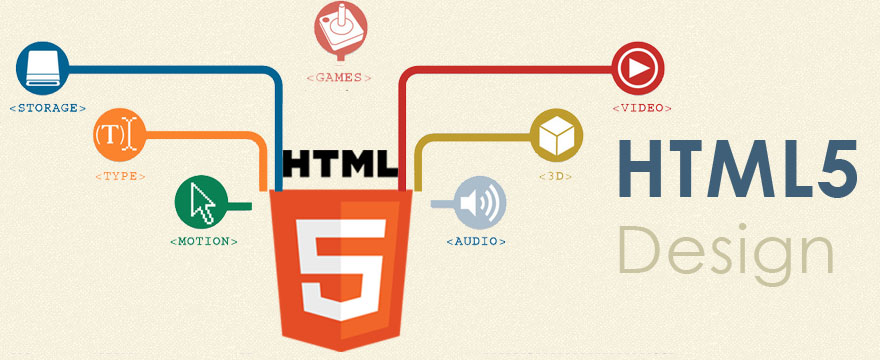
\includegraphics[width=0.8\textwidth,natwidth=610,natheight=642]{html5.jpg}
    \caption{Suíte HTML}
\end{figure}

Uma tecnologia fortemente entrelaçada com o HTML é o DOM. Tendo uma relação próxima de um para um com a marcaçaõ \autocite{howBrowsersWork}. DOM permite a interação entre documentos HTML e as demais tecnologias da WEB de uma forma fácil e padronizada.

\subsection{DOM}
%{{{

O modelo de documento de objetos (\textit{Document Object Model}) é
a representação em memória de uma árvore de elementos HTML. Esta
representação é definida por um conjunto de padrões que torna
interoperável a manipulação de elementos através de JavaScript.

A primeira versão do DOM, DOM nível zero, foi parcialmente
especificada no HTML 4 e permitia manipulação parcial dos elementos.
Foi somente com a especificação do JavaScript em 1998 que o DOM nível
1 foi especificado, permitindo a manipulação de qualquer elemento. DOM
nível 2 e 3 seguiram com melhorias nas consultas aos elementos e CSS.

\begin{figure}
\centering
\begin{verbatim}
    var elementos = document.querySelector( ".main, #sceen"  );
    var elementosB = document.querySelectorAll( "a.minhaClasse, p"  );
\end{verbatim}
\caption{Exemplo de utilização de seletores do DOM em JavaScript}
\label{fig:selectorsSample}
\end{figure}

A API de seletores (\textit{querySelector}) do DOM permite alto
nível de precisão e performance para buscar elementos. A figura
\ref{fig:selectorsSample} exemplifica a utilização dos seletores
do DOM em um documento JavaScript. O método \textit{querySelector}
seleciona o primeiro elemento em conformidade com o padrão
especificado. Já o método \textit{querySelectorAll} seleciona todos os
elementos que estão em acordo com o padrão especificado.

%}}}
%}}}
\section{CSS}
%{{{
CSS (\textit{Cascading Style Sheets}) é uma linguagem de folhas de
estilo criada por Håkon Wium Lie em 1994 com intuito de definir a
apresentação de páginas HTML. CSS, juntamente com JavaScript e HTML,
compõem as tecnologias centrais no desenvolvimento WEB tornando-se
parte da OWP; sua especificação é atualmente mantida pela W3C.

O termo \textit{Cascading} refere-se ao fato de regras serem
herdadas pelos filhos de um elemento, eliminando grande parcela de
duplicação antes necessária para estilizar uma página. Segundo
\cite{html5mostwanted} pode-se expressar regras gerais que são
"cascateadas" para muitos elementos, e então sobrescrever os elementos
específicos conforme a necessidade.

Segundo \cite[pp. 23--24]{CascadingStyleSheets}:
\begin{quote}
CSS possibilita a ligação tardia (\textit{late biding}) com
páginas HTML. Essa característica é atrativa para os publicadores
por dois motivos. Primeiramente pois permite o mesmo estilo em várias
publicações, segundo pois os publicadores podem focar-se no conteúdo
ao invés de se preocuparem-se com detalhes de apresentação.
\end{quote}

Esta ligação tardia permitiu diferenciação entre apresentação e
estrutura, sendo neste caso o CSS responsável pela apresentação. Esta
característica é uma das ideias pioneiras do SGML, motivo que tornou a
utilização do CSS tão conveniente para o desenvolvimento WEB.

Antes do CSS era impossível ter estilos diferenciados para diferentes
tipos de dispositivos, limitando a aplicabilidade dos documentos.
Com CSS também tornou-se possível que o usuário declare suas próprias
folhas de estilo, um recurso importante para acessibilidade.

Estruturalmente falando, CSS é formado por um conjunto de regras,
dentro de uma tag HTML denominada \textit{style}, que são agrupadas
por seletores em blocos de declaração. Os elementos selecionados são
denominados o assunto do seletor \autocite{cssSelectors}. Seletores tem
o intuito de definir quais partes do documento HTML serão afetadas por
determinado bloco de declaração.

A figura \ref{fig:CSSSample} exemplifica este processo. O seletor em
questão é o elemento \textit{<p>}, simbolizando todos os parágrafos. O bloco de
declaração é o que está dentro das chaves, aplicando alinhamento e
cores aos parágrafos.

\begin{figure}
\centering
\begin{verbatim}
<style>
p {
    text-align: center;
    color: red;
}
</style>
\end{verbatim}
\caption{Exemplo de Folha de Estilo}
\label{fig:CSSSample}
\end{figure}

CSS é dividido em módulos, que representam conjuntos de
funcionalidades, contendo aproximadamente 50 deles. Cada módulo evolui
separadamente, esta abordagem é preferível pois permite uma maior
entrega de novas funcionalidades visto que novos recursos não dependem
da aceitação de outros para serem disponibilizados.

Além do módulos, CSS também é organizado por perfis e níveis.

Os perfis do CSS organizam a especificação por dispositivo de
utilização. Existem perfis para dispositivos móveis, televisores,
impressoras, etc. A aplicabilidade das regras do CSS varia dependendo do
perfil. O conteúdo do elemento \textit{strong}, por exemplo, pode ser
traduzido em uma entonação mais forte em um leitor de telas, já em um
navegador convencional pode ser apresentado como negrito.

Já os níveis organizam o CSS por camadas de abstração. Os níveis
inferiores representam as funcionalidades vitais do CSS, os níveis
superiores dependem dos inferiores para construir as funcionalidades
elaboradas. %um exemplo seria legal

A primeira especificação do CSS, CSS1 (ou nível 1) foi lançada em
1996. Em 1997 foi lançado o CSS2 com o intuito de ampliar a completude
do CSS1. Em 1998 iniciou-se o desenvolvimento do CSS3 que ainda continua
em 2015. Além do nível 3 existem módulos de nível 4 no CSS, não
obstante o termo CSS3 ainda é o mais utilizado.

Apesar da clara evolução das versões do CSS, esse processo nem
sempre é linear. Em 2005 o grupo de trabalho do CSS decidiu aumentar a
restrição de suas especificações rebaixando o CSS 2.1, Seletores do
CSS3 e Texto do CSS3 de recomendações para rascunhos.

\begin{figure}
    \centering
    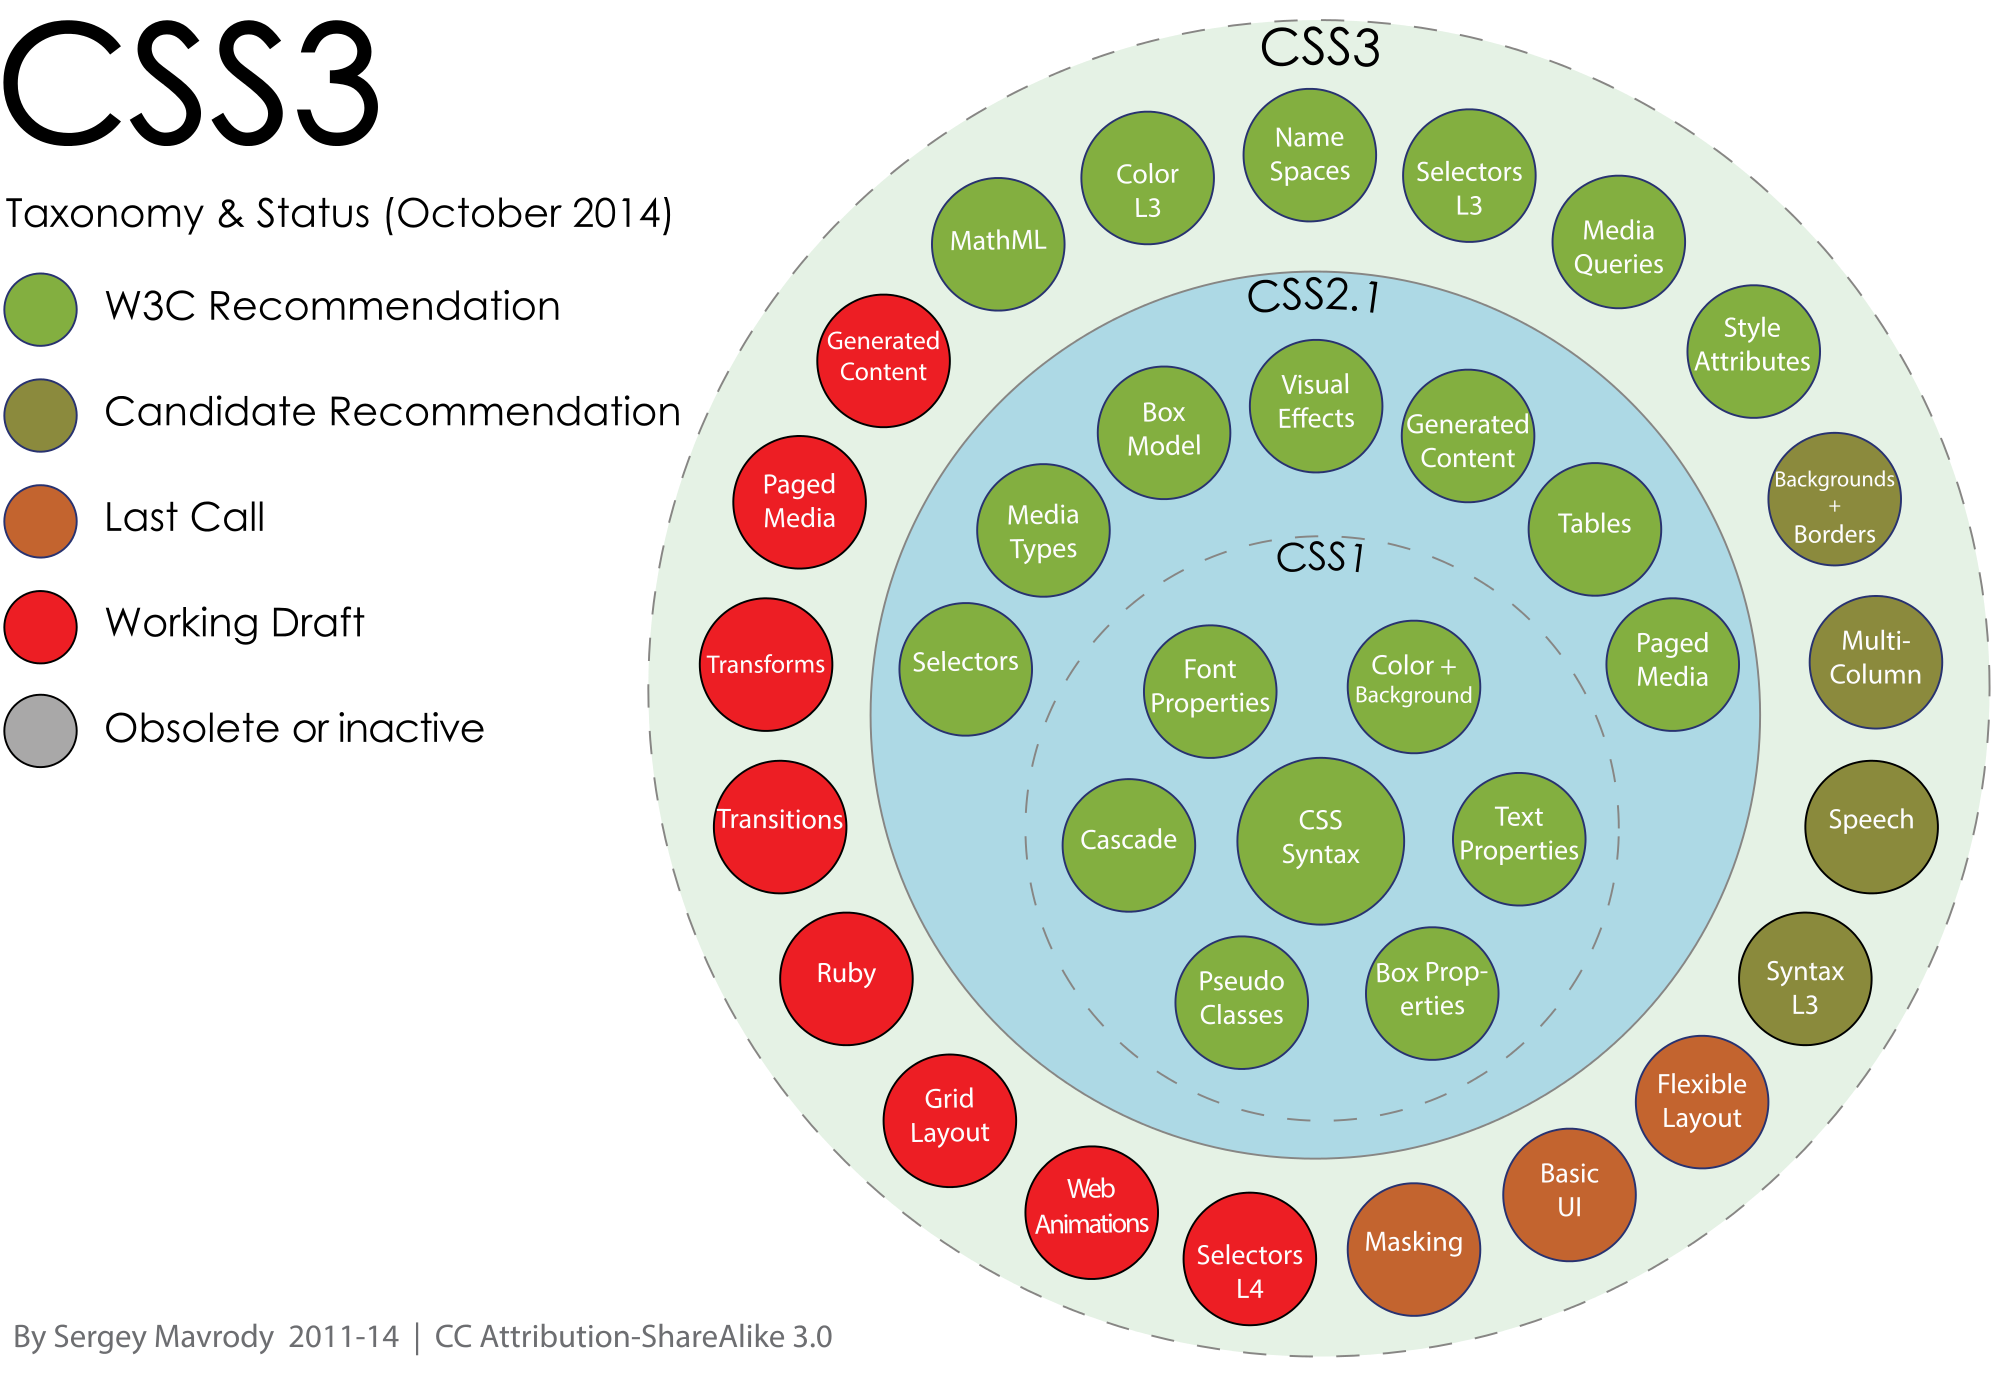
\includegraphics[width=0.8\textwidth,natwidth=610,natheight=642]{cssModules.png}
    \caption{Os módulos do CSS}
    \source{https://commons.wikimedia.org/wiki/File:CSS3\_taxonomy\_and\_status-v2.png}
\end{figure}

A última versão do CSS, o CSS3, introduziu várias funcionalidades
relevantes para jogos, como \textit{media-queries}, transições,
transformações 3D, entre outros.

\subsection{Media Queries}

Media Queries permitem aplicar regras a dispositivos específicos,
dependendo de suas capacidades, como resolução, orientação, tamanho
de tela, entre outros. A especificação prevê a possibilidade de
condicionalmente carregar arquivos JavaScript ou CSS, ou utilizar
seletores dentro do CSS de acordo com regras de Media Queries.

Esse carregamento condicional  permite implementar fluidez e
adaptabilidade de layout para diferentes resoluções. Que segundo
\cite{HTML5CrossPlatformGameDevelopment} é o mais importante aspecto do
desenvolvimento de jogos multiplataforma com as tecnologias da WEB.

\begin{figure}
\centering
\begin{verbatim}
@media only screen and (min-width: 1024px) {
    background-color: green;
}
\end{verbatim}
\caption{Exemplo de Media Query}
\label{fig:MediaQuery}
\end{figure}

A figura \ref{fig:MediaQuery} demostra a aplicação de uma regra via
seletor Media Query, aplicando o a cor de fundo para dispositivos com no
minimo 1024 pixels de resolução.

CSS nível 4 permite a utilização de media queries (\textit{Custom
Media Queries}) criados pelo usuário, com regras e definições
customizadas. A figura \ref{fig:MediaQueryCustom} demostra as novas
possibilidades de definição de media queries tanto em CSS como em
JavaScript.

\begin{figure}
\centering
\begin{verbatim}
@custom-media --narrow-window (max-width: 30em);

<script>
CSS.customMedia.set('--foo', 5);
</script>

\end{verbatim}
\caption{Exemplo de media queries customizados}
\label{fig:MediaQueryCustom}
\source{https://developer.mozilla.org/en-US/docs/Web/CSS/MediaQueries}
\end{figure}

%falar de tamanhos absolutos vs relativo
%Unidades vw e vh para tamanho do viewport

\subsection{Transições}

Transições são uma forma de adicionar animações em uma página
web. Estas animações são compostas por um estado inicial e um final.
A especificação de transições permite grande controle sobre seus
estados, habilitando o desenvolvedor a controlar o tempo de execução,
os estados intermediários, e efeitos aplicados uma transição.

Para utilizar transições, assim omo em uma máquina de estados,
precisamos identificar estados e ações. Estados são seletores do CSS
e ações são modificações realizadas entre esses dois seletores CSS
\autocite{html5mostwanted}.

Transições são interessantes em jogos, especialmente pois muitos
navegadores suportam aceleração de GPU (Unidade de processamento
gráfico) para estas operações. Isso garante grandes benefícios de
performance sobre implementações diretamente em JavaScript.

Segundo \cite{html5mostwanted} transições nos permitem construir jogos
degradáveis pois os interpretadores de CSS são amigáveis; se eles
encontrarem propriedades desconhecidas eles simplesmente as ignoram e
continuam a funcionar.

\begin{figure}
\centering
\begin{verbatim}
div {
    width: 100px;
    height: 100px;
    background: red;
    transition: width 2s;
}

div:hover {
    width: 300px;
}

\end{verbatim}
\caption{Exemplo de transição}
\label{fig:CSSTransition}
%\soruce{http://www.w3schools.com/CSS/css3\_transitions.asp}
\end{figure}

A figura \ref{fig:CSSTransition} demostra a utilização de uma
transição de tamanho em uma \textit{div} quando o mouse está sobre o
elemento. No período de 2 segundos a largura da \textit{div} vai de 100
pixels ara 300 pixels.

Atualmente um conjunto finito de propriedades podem ser animadas
com transições, e essas lista tende a mudar com o tempo, cabe ao
desenvolvedor assegurar-se que determinada propriedade está disponível
\autocite{mdnTransitions}.

\subsection{Transformações 3D}

Transformações é outra tecnologia do CSS3 que permite grande
flexibilidade na construção de jogos. Transformações permitem que
elementos sejam traduzidos, rotacionados, escalados e distorcidos em um
espaço de duas dimensões \autocite{html5mostwanted}.

A transformação demonstrada na figura \ref{fig:CSSTransform} escala o
tamanho do elemento com a classe (\textit{test}) para vinte porcento a
mais do seu tamanho original. Perceba também os comandos repetidos com
o prefixo ms e WebKit. Esse tipo de abordagem é comum para tecnologias
que não passam de rascunhos na especificação.

Assim como transições, as transformações são muitas vezes aceleradas
via GPU incrementando a performance de animações criadas com a tecnologia.

\begin{figure}
\centering
\begin{verbatim}
<style>
.test:hover
{
        -webkit-transform: scale(1.2);
        -ms-transform: scale(1.2);
        transform: scale(1.2);
}
</style>
\end{verbatim}
\caption{Exemplo de transformação}
\label{fig:CSSTransform}
\end{figure}

\subsection{CSS 4}

Apesar de o termo CSS 4 ser bastante utilizado, o grupo de trabalho do CSS
não considera mais a existência de versões, como foi até o CSS3.
Não obstante existem recursos cuja especificação está avançada e não estavam presentes
no CSS 3 quando este foi lançado, dentre estas funcionalidades inclui-se:

\begin{itemize}
\item Suporte a variáveis no CSS
\item Media queries customizadas
\item Funções de cores como: color(), hwb() e gray()
\item Suporte a filtros
\end{itemize}

Recursos recentes do CSS muitas vezes não estão presentes nos
navegadores, não obstante muitos deles são interessantes no contexto
de desenvolvimento de jogos, como o suporte a variáveis.

O projeto cssnext http://cssnext.io/ é uma iniciativa para permitir a
utilização dos recentes recursos do CSS mesmo sem os mesmos estarem
implementados nos navegadores. O projeto funciona compilando o código
não suportado em algo compatível com versões para as versões
implementadas pelos navegadores.

Além da apresentação, recurso vital para jogos, e aplicativos web em
geral, é a iteratividade. Com as tecnologias da WEB esta iteratividade
é atingida através do JavaScript.
%}}}
\section{JAVASCRIPT}
%{{{

EMACScript, melhor conhecida como JavaScript, criada por Brendan Eich em
1992, é a linguagem de script da Web. Devido a tremenda popularidade
entre comunidade de desenvolvedores a linguagem foi abraçada pela W3C e
atualmente é um dos componentes da Open Web.

As definições da linguagem são descritas na especificação ECMA-262.
Esta possibilitou o desenvolvimento de outras implementações além da
original (SpiderMonkey) como o Rhino, V8 e TraceMonkey; bem como
outras linguagens similares como JScript da Microsoft e o ActionScript
da Adobe.

Segundo a \cite{ecmaSpecificaton}:
\begin{quote}
Uma linguagem de script é uma linguagem de programação que é
usada para manipular e automatizar os recursos presentes em um dado
sistema. Nesses sistemas funcionalidades já estão disponíveis
através de uma interface de usuário, uma linguagem de script é
um mecanismo para expor essas funcionalidades para um programa
protocolado.
\end{quote}

No caso de JavaScript na web, os recursos manipuláveis são o conteúdo
da página, elementos HTML, elementos de apresentação,
a própria janela do navegador e variados outros recursos que tem
suporte adicionado por novas especificações.

A intenção original era utilizar o JavaScript para dar suporte aos já
bem estabelecidos recursos do HTML, como para validação, alteração
de estado de elementos, etc. Em outras palavras, a utilização do
JavaScript era opcional e as páginas da web deveriam continuar
operantes sem a presença da linguagem.

Não obstante, com a construção de projetos Web cada vez mais complexos, as
responsabilidades delegadas ao JavaScript aumentaram a ponto que a
grande maioria dos sistemas web não funcionarem sem ele.
JavaScript não evoluiu ao passo da demanda e muitas vezes carece de
definições expressivas, completude teórica, e outras características
de linguagens de programação mais bem estabelecidas, como o C++ ou
Java \autocite{crossPlatformMobileGame}.

A última do JavaScript, o JavaScript 6, é um esforço nessa direção.
JavaScript 6 ou EMACScript Harmonia, contempla vários conceitos de
orientação a objetos como classes, interfaces, herança, tipos, etc.
Não obstante o suporte ao JavaScript 6 é apenas parcial em todos
os navegadores. O site http://kangax.github.io/compat-table/es6/
apresenta um comparativo de suporte das funcionalidades do JavaScript.

Segundo \cite{ecmaSupport} o suporte no início de 2015 era o seguinte:

\begin{itemize}
    \item Chrome: 30\%
    \item Firefox: 57\%
    \item Internet Explorer : 15\%
    \item Opera: 30\%
    \item Safari: 19\%
\end{itemize}

Estes esforços de padronização muitas vezes não são rápidos
o suficiente para produtores de software web, demora-se muito até
obter-se um consenso sobre quais as funcionalidades desejadas em
determinada versão e seus detalhes de implementação. Além da
espera por especificações, uma vez definidas, é necessário que os
navegadores especificado.

O projeto babel https://github.com/babel/babel é um compilador de
JavaScript 6 para JavaScript 5. Permitindo que, mesmo sem suporte, os
desenvolvedores possam usufruir dos benefícios da utilização do
JavaScript 6 durante o tempo de desenvolvimento, gerando código em
JavaScript 5 para rodar nos navegadores.

Alternativamente, existe uma vasta gama de conversores de código
(\textit{transpilers}) para JavaScript; possibilitando programar
em outras linguagens posteriormente gerando código JavaScript
\footnote{Uma lista das tecnologias para converter código HTML pode ser encontrada nos apêndices}.
Entretanto, essa alternativa tem seus pontos fracos, necessita-se
de mais tempo de depuração, visto que o JavaScript gerado não é
conhecido pelo desenvolvedor, e provavelmente o código gerado não
será tão otimizado, nem utilizará os recursos mais recentes do
JavaScript.

Mesmo com suas fraquezas amplamente conhecidas, JavaScript está
presente em praticamente todo navegador atual. Sendo uma espécie de
denominador comum entre as plataformas. Essa onipresença torna-o
integrante vital no processo de desenvolvimento de jogos multiplataforma
em HTML5. Vários títulos renomeados já foram produzidos que fazem
extensivo uso de JavaScript, são exemplos: Candy Crush Saga, Angry
Birds, Dune II, etc.

Jogos Web são geralmente escritos na arquitetura cliente servidor,
JavaScript pode rodar em ambos estes contextos, para tanto, sua
especificação não define recursos de plataforma. Distribuidores do
JavaScript complementam a o JavaScript com recursos específicos para
suas plataformas alvo. Por exemplo, para servidores, define-se objetos como:
console, arquivos e dispositivos; no contexto de cliente,
são definidos objetos como: janelas, quadros, DOM, etc.

Para o navegador o código JavaScript geralmente é disposto no elemento
script dentro de arquivos HTML. Quando os navegadores encontram esse
elemento eles fazem a requisição para o servidor e injetam o código
retornado no documento, e a não ser que especificado de outra forma,
iniciam sua execução.

\subsection{JAVASCRIPT 7}

Antes da finalização da especificação 6, algumas funcionalidades
do JavaScript 7 já haviam sido propostas. Na página
https://github.com/tc39/ecma262 pode-se conferir os itens propostos e
seu estágio de evolução. A figura \ref{fig:ecma7} é a tabela de
funcionalidades sugeridas e seu estágio no caminho da especificação.

Alguns dos recursos esperados para o JavaScript 7 são: guards,
contratos e concorrência no laço de eventos \autocite{ecma7}.

\begin{figure}
    \centering
    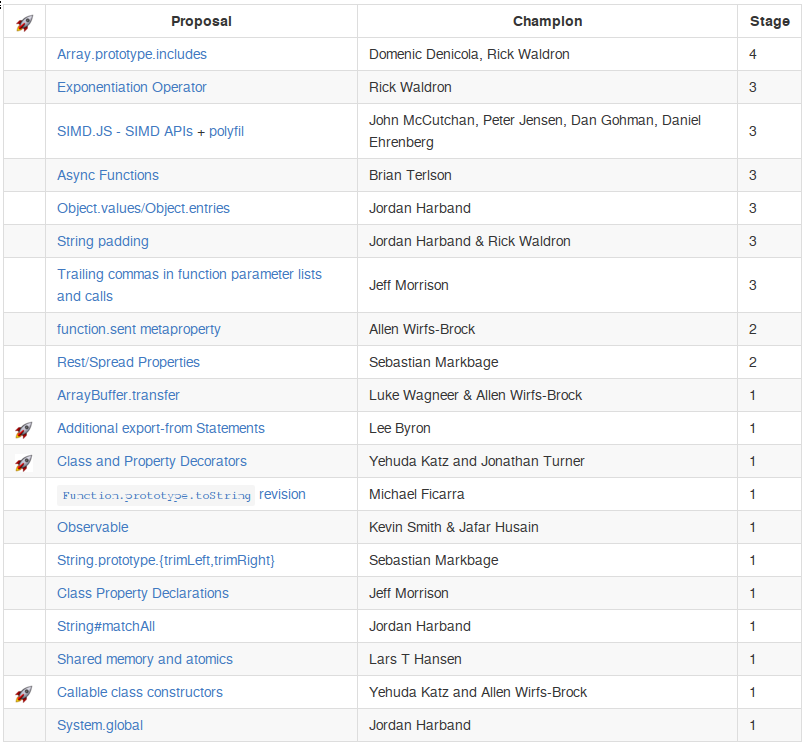
\includegraphics[width=0.8\textwidth,natwidth=610,natheight=642]{ecma7.png}
	\caption{Propostas do ECMA 7}
	\source{https://github.com/tc39/ecma262}
    \label{fig:ecma7}
\end{figure}

\subsection{ASM.JS}% o correto é asm.js

Asm.js é um subconjunto da sintaxe do JavaScript a qual permite
grandes benefícios de performance quando em comparação com
JavaScript normal. Entretanto, não é trivial escrever código em
asm.js e geralmente a criação de código asm.js é feita através
da conversão de outras linhagens como C. O projeto Emscripten
https://github.com/kripken/emscripten pode ser utilizado para gerar
código em asm.js é utilizado pelo motor de jogos Unity 3D e Unreal.

No contexto dos jogos performance é um fator de extrema importância
asm.js se destaca por utilizar recursos que permitam otimizações
antes do tempo (\textit{ahead of time optimizations}). Grade parcela
da performance adicional, em relação ao JavaScript, é devido a
consistência de tipo e a não existência de um coletor de lixo
(\textit{garbage collector}) a memória é gerenciada manualmente
através de um grande vetor. Esse modelo simples desprovido de
comportamento dinâmico, sem alocação e desalocação de memória,
apenas um bem definido conjunto de operações de inteiros e flutuantes
possibilita grade performance e abre espaço para otimizações.

O desenvolvimento do asm.js iniciou-se no final de 2013 não obstante a
maioria dos navegadores não implementam ou implementam parcialmente o
rascunho. O motor JavaScript da Mozilla, SpiderMonkey, é a exceção,
implementando a grande maioria dos recursos do asm.js.

\subsection{WEB Assembly}
%{{{
Web Assembly é uma tecnologia que pretende definir um formato de
máquina da Web. A tecnologia ainda está em seus estágios iniciais
de desenvolvimento, nem conta com um grupo de trabalho. Não obstante,
sabe-se que WEB Assembly irá permitir que outras linguagens além do
JavaScript gerem código binário que rode nos navegadores com grande
ganhos de performance e flexibilidade.

Além da versão binária, otimizada para performance, uma versão em
texto também está prevista, ideal para desenvolvimento e depuração.
Bibliotecas aplicações que requeiram grande performance como
motores de física, simulações e jogos em geral vão se beneficiar
substancialmente com o Web Assembly.

A iniciativa do Web Assembly está sendo desenvolvida pelo Google,
Microsoft, Mozilla, entre outros, tornando a proposta uma possibilidade
promissora. Seu objetivo não é substituir o JavaScript, outrossim
habilitar que aplicações que necessitem de grande performance possam
ser inclusas na WEB. A ideia do WEB Assembly é uma continuação
do trabalho do asm.js, uma forma de trazer performance similar a
nativa eliminando grande parte das abstrações que o traz JavaScript
embutidas.

Visto que os desenvolvedores de motores JavaScript terão que colocar
o código do Web Assembly na mesma base que o do JavaScript as
expectativas são de que o JavaScript consiga aproveitar partes
da implementação do Web Assembly incrementando a performance do
JavaScript.

A aplicabilidade do Web Assembly em jogos em produção ainda
é praticamente nula. Até então apenas um polyfill do Web
Assembly está disponível e pode ser encontrado no seguinte link
https://github.com/Web\_Assembly/polyfill-prototype-1. Mas conforme a
especificação evolui a probabilidade é que as empresas interessadas
implementem a especificação em seus navegadores e os desenvolvedores
de jogos comecem a integrar a tecnologia em suas aplicações.

%}}}
\subsection{Web Animations}
%{{{

Web Animations é uma especificação em rascunho que define uma forma
imperativa de manipular animações através de JavaScript. Como
demostrado na figura \ref{fig:webAnimations} a tecnologia vai permitir
manipular as animações de elementos do DOM, com a possibilidade de 
filtrar por tipo de animação, alterar a taxa de
animações, o tempo de execução, entre outras propriedades de uma
forma dinâmica - através de scripts.

Visto que Web Animations lida diretamente com o DOM, animações podem
ser aplicadas para SVG além de CSS, servindo como uma tecnologia para
unificar animações.

Grande controle sobre animações é desejável para os jogos, não obstante,
visto que a especificação é muito nova somente o Google Chrome a implementa.
A biblioteca https://github.com/web-animations/web-animations-js serve
como polyfill para os demais navegadores.

\begin{figure}
    \centering
    \begin{verbatim}
elem.getAnimations().filter(
  animation =>
    animation.effect instanceof 
    KeyframeEffectReadOnly &&
    animation.effect.getFrames().some(
      frame => frame.hasOwnProperty('transform')
    )
).forEach(animation => {
  animation.currentTime = 0;
  animation.playbackRate = 0.5;
});
    \end{verbatim}
	\caption{Exemplo de utilização de WEB Animatios}
	\source{http://www.w3.org/TR/WEB-animations/}
    \label{fig:webAnimations}
\end{figure}

O site http://web-animations.github.io/web-animations-demos/ contém uma
coleção de animações utilizando a tecnologia.

%\end{draft}
%}}}
%}}}
\section{NAVEGADORES}
%{{{
Navegadores são aplicações, onde as tecnologias da OWP são
interpretadas e geram um conteúdo útil para os usuários.

Navegadores geralmente são os clientes em uma arquitetura cliente
servidor. O servidor geralmente é um servidor WEB que disponibiliza
páginas HTML para o navegador processar. A comunicação entre o 
navegador e o servidor se dá através da troca de mensagens no protocolo
HTTP.

Nos navegadores os usuários necessitam saber o endereço de determinado
servidor, ou utilizar buscadores para auxiliá-los. Este é um processo
árduo para a plataformas móveis pois necessitam maior interação
do usuários e não são “naturais” se comparado ao modo 
de consumir aplicativos nestas mesmas plataformas – simplesmente
adquirindo o aplicativo na loja e abrindo-o no sistema operacional.
Algumas formas de contornar este problema serão descritos nas tecnologias offline.

Uma vez localizado o endereço o cliente manda uma mensagem em http requisitando 
o conteúdo de determinado endereço.
O servidor responde a mensagem HTTP com um documento HTML
 e o cliente, ao receber, começa o processo de renderização. A renderização consiste
na decodificação de um documento em HTML para sua representação
memória e posterior pintura no espaço de tela do navegador. Para
concluir o processo de renderização o navegador pode requisitar outros
arquivos a fim de completar a experiência desejada para o endereço
em questão.

O processo de renderização é complexo e a grande maioria dos navegadores
confia em bibliotecas especializadas para efetuar este trabalho.

Alguns motores de renderização incluem:

\begin{itemize}
    \item Blink: Utilizada no Chromium e projetos relacionados, Opera
    \item Gecko: Utilizada nos produtos da Mozilla
    \item KHTML: Utilizada no navegador Konkeror, esta serviu de base para o Blink
    \item WebKit: Utilizada no Safari e versões antigas do Google Chrome.
\end{itemize}

Para interpretar HTML o motor WebKit utiliza a biblioteca Bison, já o
Gecko utiliza uma biblioteca própria \autocite{howBrowsersWork}.

O código que é executado no lado do servidor geralmente é terceirizado pelos navegadores.
As bibliotecas que executam JavaScript são os motores de JavaScript.

\begin{itemize}
    \item SpiderMonkey: Primeiro motor, desenvolvido por Brendan Eich, escrito em C++
    \item Rhino: Criada pela Netscape, escrito em Java
    \item Nitro: Criada pela Apple
    \item V8: Criada pelo Google
    \item TraceMonkey: Criada pela Mozilla
\end{itemize}

O suporte ao HTML vem crescendo com o tempo, o site HTML5Test
http://html5test.com/about.html, oferece um placar atualizado
dinamicamente, conforme utilização dos navegadores, sobre os recursos
do HTML.

A figura \ref{fig:audioCodecs} apresenta o gráfico de suporte por
versões de navegadores em dezembro de 2015.

\begin{figure}
    \centering
    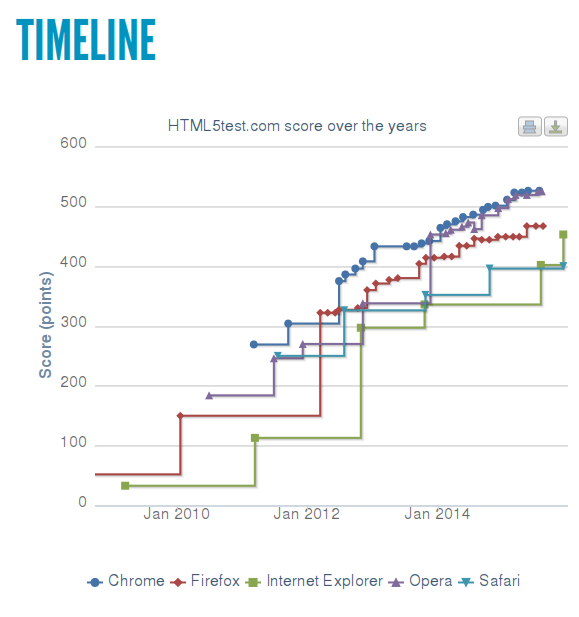
\includegraphics[width=0.8\textwidth,natwidth=610,natheight=642]{htmlSupport.png}
	\caption{Suporte das especificações do HTML nos navegadores}
    \label{fig:htmlSupport}
\end{figure}

%}}}
\section{ANDROID}
%{{{
\begin{draft}
É um sistema operacional open-source desenvolvido pela Google. Utiliza
o kernel Linux . Softwares para Android são geralmente escritos em Java
e executados através da máquina virtual Dalvik.

É similar a máquina virtual Java, mas roda um formato de arquivos
diferenciado (dex), otimizados para consumir pouca memória, que
são agrupados em um único Android Package (apk) Android permite a
renderização de documentos HTML através de sua própria API WEBVIEW.
Ou através do navegador disponibilizado por padrão, ou outros de
terceiros como o Google Chrome, Firefox, Opera, etc.

No quesito jogos para dispositivos móveis é preferível disponibilizar
os jogos através da interface nativa pois dá a sensação de
continuidade para com os demais aplicativos instalados no dispositivo.
\end{draft}
%}}}
\section{DETECÇÃO DE RECURSOS}
%{{{
Visto que nenhum navegador implementa as especificações HTML
completamente cabe ao desenvolvedor detectar os navegadores que não
comportam as necessidades tecnológicas dos aplicativos que cria. Ao
deparar-se com uma funcionalidade faltante o desenvolvedor tem duas
possibilidades: notificar o usuário sobre o problema ou utilizar
polyfills.

Polyfills são recursos que simulam uma funcionalidade não
disponível nativamente nos navegadores. A biblioteca Gears
https://developers.google.com/gears é um exemplo. Gears
serve para prover recursos de Geolocalização para navegadores que
não implementam a especificação do HTML5. 

Essa capacidade de suportar tecnologias que não estão ainda
disponíveis (ou nunca estarão no caso de dispositivos legados)
através de polyfills é uma das características que faz a WEB uma
plataforma de tão grande abrangência. Novas tecnologias são criadas a
todo o momento; entretanto, o suporte a essas funcionalidades geralmente
não acompanham o passo das inovações. E ainda assim os usuários
podem se beneficiar de uma taxa substancial delas através de polyfills.

Algumas funcionalidades do HTML, como geolocalização e vídeo
foram primeiramente disponibilizadas através de plugins. Outras
funcionalidades, como o canvas, podem ser totalmente emuladas via
JavaScript \autocite{diveIntohtml}.

Detectar suporte aos variados recursos do HTML5 no navegador
pode ser uma tarefa entediante. É possível implementar testes para
cada funcionalidade utilizada abordando os detalhes de implementação
de cada uma ou então fazer uso de alguma biblioteca especializada
neste processo. O Modernizr é uma opção open-source deste tipo de
biblioteca, este gera uma lista de booleanos sobre grande variedade dos
recursos HTML5, dentre estes, geolocalização, canvas, áudio, vídeo e
armazenamento local.

A quantidade de especificações que um aplicativo complexo como um jogo
utiliza pode ser bem grande, e muitas vezes é difícil dizer qual quais
navegadores implementam o quê. Uma boa referência do suporte a recursos
nos navegadores é o site http://caniuse.com/.

%}}}
\section{RENDERIZAÇÃO}
%{{{

Renderização é parte fundamental de muitos jogos. As tecnologias atualmente existes são o SVG e Canvas.

\subsection{SVG}
%{{{
\begin{draft}
SVG (\textit{Gráficos de vetores escaláveis}), é uma linguagem
baseada em XML especializada na criação de vetores bidimensionais
\autocite{html5mostwanted}. Por usar XML SVG permite a utilização da
API do DOM para manipular os elementos.

Entre os benefícios do SVG encontram-se:
\begin{itemize}
\item Não há diferença de qualidade em resoluções pois os vetores são escaláveis;
\item Suporta animações nativamente;
\item Conta com integração através da api do DOM. Tornando simples a integração com as outras tecnologias da web.
\end{itemize}

Um aspecto negativo do SVG é que é muito difícil atingir a
perfeição na posição dos pixels, por ser uma linguagem vetorizada
\autocite{html5mostwanted}.

\end{draft}
\begin{figure}
\centering
\begin{verbatim}

<svg height="100" width="100">
  <circle cx="50" cy="50" r="40" stroke="black" stroke-width="3"/>
  Sorry, your browser does not support inline SVG.
</svg>

\end{verbatim}
\caption{Círculo em SVG.}
\end{figure}
%}}}
\subsection{CANVAS}
%%{{{
\begin{draft}
O elemento \textit{canvas} define uma camada de mapa de bits em documentos
HTML que pode ser usada para criar diagramas, gráficos e animações
2D. Foi criada pela Apple em 2004 para renderizar elementos de interface
no Webkit, logo foi adotado por outros navegadores e se tornou um
padrão.

Em um documento HTML, canvas é um retângulo onde pode-se usar
JavaScript para desenhar \autocite[pp. 113]{diveIntohtml}. Manipular o
retângulo é uma analogia de como desenhar manualmente, move-se
o "lápis" para o local desejado, e traça-se os pontos onde a linha
deve percorrer - similar ao planejamento. E desenha-se efetivamente,
preenchendo os pontos demarcados.

Os desenhos do canvas não podem ser acessados via dom nem serem manipulados via CSS, todas as modificações necessárias devem ser feitas via JavaScript.

Segundo \cite{gwt} uma característica importante deste [canvas]
elemento é que ele consegue redimensionar seu conteúdo para adequar à
resolução do navegador do usuário.

O canvas até aqui descrito trata-se de sua forma, ou contexto 2D. A
especificação 3D do canvas é o WebGl.

\end{draft}
%}}}
\subsection{WEBGL}
%{{{
\begin{draft}

WebGL é uma API JavaScript otimizada desenhar gráficos em três dimensões.
WebGL é ideal para a criação de ambientes virtuais, jogos e simulações.
Por ser uma tecnologia da OWP WebGL foi especificado para funcionar
nativamente nos navegadores sem a ajuda de plugins ou ferramentas de terceiros.

WebGL foi desenvolvido baseando-se na especificação OpenGL, que trata
de definir como renderizar gráficos multiplataforma, especificamente
OpenGL ES 2.0, uma versão do OpenGL otimizada para dispositivos
móveis. O órgão que especifica o WebGL é o mesmo que especifica o
OpenGL, o grupo sem fins lucrativos Kronos. Os primeiros rascunhos do
WebGL iniciaram em 2006, não obstante o grupo de trabalho não foi
formado até 2009. E a primeira versão do foi lançada em 2011.

Apesar de ter sido desenvolvido com foco em 3D, WebGL pode ser
igualmente utilizado para criação de gráficos em duas
dimensões\autocite[pp. 6]{3daps}. O elemento do DOM que provê a
interface do WebGL é o canvas, no contexto 3D. Essa integração com
o DOM via tag canvas permite que o WebGL seja manipulado assim como os
demais elementos HTML.

Especificação é composta por uma API de controle em JavaScript e o
processamento shaders do lado da GPU (Central de processamento gráfico).

\subsection{Shaders}

Shaders são scripts que definem níveis de cor ou efeitos especiais
sobre um modelo 2D ou 3D. Contam com grande performance, possibilitando
conteúdo em tempo real (como no caso de jogos) por executarem dentro
da GPU. São utilizados no cinema, em imagens geradas por computadores e
vídeo games.

Existem dois shaders principais, de vértices e fragmentos.
Shaders de vértices são chamados para cada vértice sendo desenhado
definindo suas posições e shaders de fragmentos a cor para cada pixel
a ser desenhado \autocite[pp.15]{3daps}.

\cite{html5mostwanted} cita que conforme a habilidade do desenvolvedor
aumenta, mover funções antes delegadas ao JavaScript para os shaders
pode aumentar a performance e oferecer uma ampla coleção de efeitos e
realismo.

Um site interessante para explorar exemplos WebGL avançados é o blog
http://learningwebgl.com que conta com tutoriais cobrindo áreas como
diferentes tipos de iluminação, carregamento de modelos em JSON,
gerenciando eventos do mouse e teclado; e como renderizar uma cena WebGL
em uma textura \autocite[pp.42]{3daps}.

Apesar da relevância, WebGL não foi utilizado no protótipo pois
ainda não está completamente suportado em navegadores populares como
o Firefox e a grande curva de aprendizado do WebGL puro é muito grande
para se encaixar no escopo deste projeto.

Uma tecnologia que se integra profundamente como ambientes virtuais
em três dimensões criados via OpenGL é o WebVR.
\end{draft}
%}}}
%}}}
\subsection{WEBVR}
%{{{
Segundo \cite{virtualReality} realidade virtual é uma experiência em
que o usuário é efetivamente imerso em um mundo virtual responsivo.
Realidade virtual é uma área nem tão nova mas que recebeu interesse
renovado recentemente. Isso se dá, pelo menos me parte, pela
massificação dos dispositivos móveis inteligentes. O hardware
necessário para fornecer uma experiência minimamente viável como
acelerômetros, câmeras e telas de alta resolução está disponível
em praticamente todos os dispositivos comercializados.

Realidade virtual é uma área de grande interessa para os produtores
de jogos, pois pode oferecer alto nível de imersão nos já
interativos e desafiadores ambientes dos jogos.

A WebVR é uma especificação que pretende trazer os benefícios
da realidade virtual para dentro do mundo da WEB. Em termos simples
a especificação define uma forma de traduzir movimentos de
acelerômetros e outros sensores de posição e movimentos para dentro
do contexto de uma um contexto 3D através de JavaScript.

Atualmente a especificação do WebVR se encontra em fase de rascunho e
as últimas versões do Firefox, e versões compiladas manualmente do
Google Chrome já permitem a utilização.
%}}}
\section{WebCL}
%{{{
É uma API em JavaScript para o recursos de OpenCL que permitem
computação paralela com grandes ganhos de performance. Aplicativos
como motores de física e renderizadores de imagens, ambos relevantes
para os jogos, podem se beneficiar grandemente de processamento feito em
paralelo, possivelmente na GPU. OpenCL é um framework para escrever
programas que funcionem em plataformas com diversas unidades de
processamento, assim como WebGL e WebCL é especificada e desenvolvida
pelo grupo Kronos.

A primeira versão da especificação foi no início de 2014 mas até
então nenhum navegador implementa o definido.
%}}}
\section{CODECS}
%{{{

Codec é o algoritmo usado para codificar e decodificar vídeo ou
áudio em um conjunto de bits \autocite{diveIntohtml}. O termo Codec é
um acrônimo, significando o processo de codificar um fluxo de dados
para armazenamento e decodificá-lo para ser consumido. O objetivo dos
codecs é diminuir o tamanho dos arquivos com a menor perda de qualidade
possível, para isso os codecs utilizam de várias estratégias de
compressão ou descarte de dados; podendo rodar tanto em hardware quanto em
software.

O funcionamento de codecs pode variar muito, conforme as estratégias de
compressão utilizadas, a quantidade de bits por segundo, entre outros
fatores. Visto que os algoritmos de compressão podem adquirir grande
complexidade muitos codecs são encobertos por licenças
que limitam sua utilização. Não obstante, também existem opções
livres de patentes e licenças.

Após ter sido codificado um fluxo de dados é armazenado em um
contêiner. Contêiners são um padrão de metadados sobre as informações
codificadas de modo a possibilitar que outros programas consigam
interpretar estas informações de forma padronizada. Assim como
codecs existem contêiners livres e com restrições de licença.

O suporte a codecs e contêiners na WEB varia de navegador para
navegador, de acordo com as preferências mercadológicas, técnicas
ou filosofias das empresas por trás dos navegadores. Segundo
\cite{diveIntohtml} não existe uma única combinação de contêiner e
codecs que funcionem em todos os navegadores.


%}}}
\section{ÁUDIO}
%{{{
\begin{draft}
Áudio é um componente vital para oferecer imersão e feedback aos
usuários de jogos. O componente de áudio é especialmente útil para
jogos de ação \autocite{browserGamesTechnologyAndFuture}. Efeitos de
som e música podem servir como parte da mecânica do jogo.

Abaixo segue uma lista dos codecs mais comuns em áudio:

\end{draft}
\begin{itemize}
    \item MP3: comummente utilizado mas não é livre de patentes
    \item ACC: avançado mas também conta com problemas de patentes
    \item Vorbis: livre de patentes
\end{itemize}

A figura \ref{fig:audioCodecs} é um comparativo interessante sobre os
formatos existentes, considerando o fator taxa de bits versus qualidade.

\begin{figure}
    \centering
    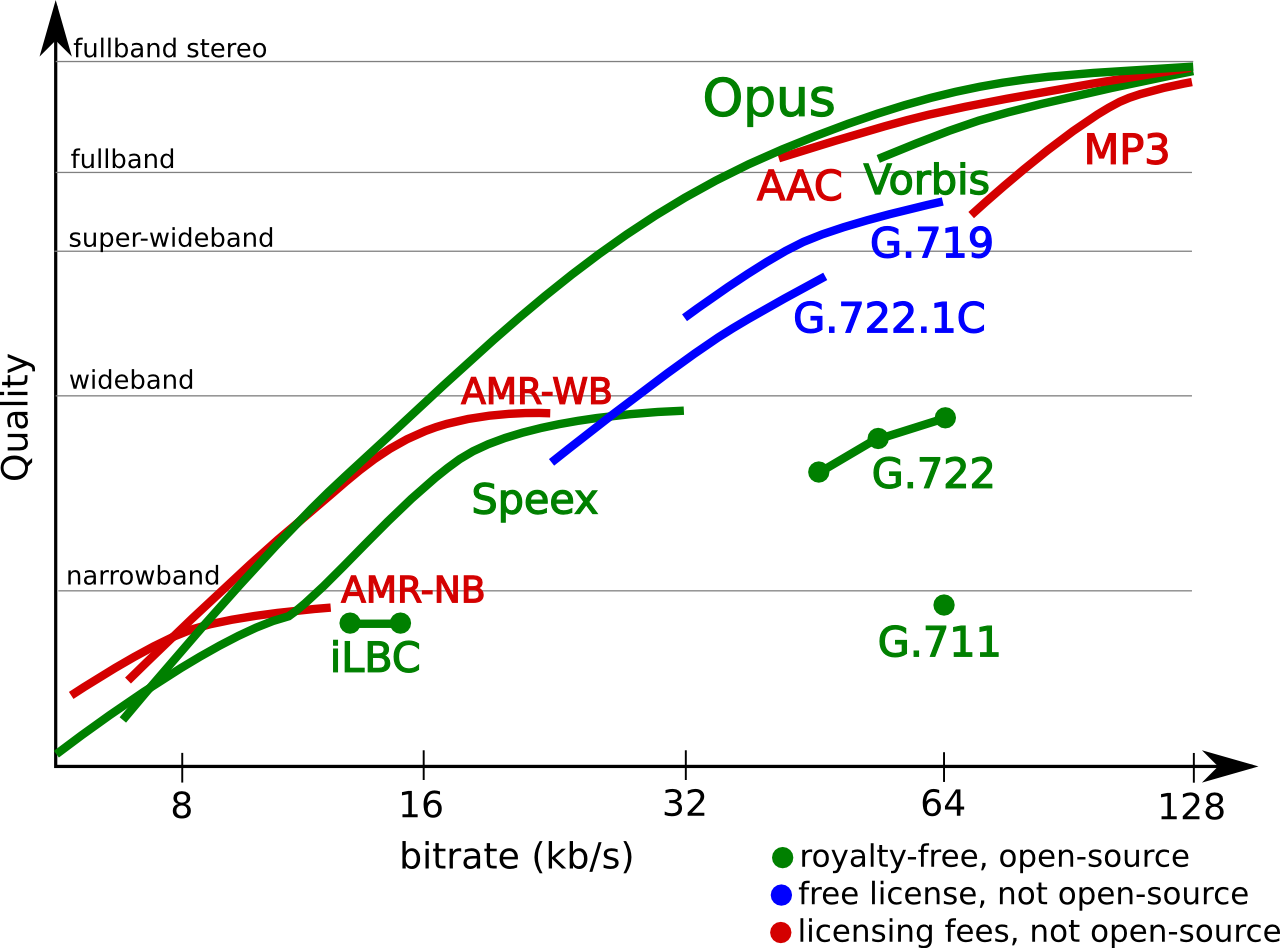
\includegraphics[width=0.8\textwidth,natwidth=610,natheight=642]{codec.png}
	\caption{Comparação de codecs de áudio}
    \label{fig:audioCodecs}
\end{figure}

HTML5 especifica duas formas de utilizar utilizar áudio na WEB.
Através do elemento HTML áudio ou através da API JavaScript de áudio.

\subsection{TAG ÁUDIO}

A tag \textit{audio} define um som dentro de um documento HTML. Quando o
elemento é renderizado pelos navegadores, ele carrega o conteúdo que
pode ser reproduzido pelo programa dentro do navegador.

\begin{figure}
\centering
\begin{verbatim}
<audio controls>
<source src="horse.ogg" type="audio/ogg">
<source src="horse.mp3" type="audio/mpeg">
Your browser does not support the audio element.
</audio>
\end{verbatim}
\caption{Exemplo de utilização da tag áudio}
\label{fig:htmlAudio}
\source{http://www.w3schools.com/HTML/HTML5\_audio.asp}
\end{figure}

A imagem \ref{fig:htmlAudio} demonstra a utilização da tag
\textit{audio}. Os elementos \textit{source} demonstrados na figura
referenciam a arquivos de áudio contendo um contêiner e codec
específico, mais de um elemento \textit{source } por áudio é
necessário para dar suporte aos diferentes navegadores.

A especificação declara que todo o conteúdo dentro de uma tag áudio
(e vídeo também), que não sejam tags \textit{source}, sejam ignoradas
pelo navegador. O que permite que seja adicionada marcação de reserva
para tratar os casos de quando não existe suporte a tag \textit{audio}
no navegador.

O objetivo inicial da tag \textit{audio} é reproduzir um som e parar.
Ideal para ouvir música, como um som de fundo. Entretanto, a tag
\textit{audio} não é o suficiente para comportar aplicações de
áudio complexas \autocite{audioApiSpec}. A grande maioria de jogos
muitas vezes precisam lançar múltiplos sons derivados de ações
de usuário e outros eventos, nestes casos a API de áudio é mais
adequada.

\subsection{API DE ÁUDIO}
\begin{draft}

É uma interface experimental (ainda em rascunho) em JavaScript para
criar e processar áudio. O objetivo da especificação é incluir
capacidades encontradas em motores de jogos modernos e também permitir
o processamento, mistura e filtragem, funcionalidades que estão
presentes nas aplicações de processamento de áudio modernas para
desktop \autocite{audioApiSpec}.

A API especificada provê uma interface para manipular nodos de
áudio que podem ser conectados permitindo refinado controle sobre os
efeitos sonoros. O processamento se dará primeiramente em uma cada
inferior (tipicamente código Assembly / C / C++), mas síntese e
processamento em JavaScript também será suportado \autocite{audioApiSpec}.

Essa tecnologia é muito mais nova do que a tag áudio. Diferentemente
dos demais navegadores o Internet Explorer não dá nenhum nível de
suporte a API. O polyfill https://github.com/shinnn/AudioContext-Polyfill
suporta as partes básicas da API e pode ser utilizada nos casos onde 
não existe suporte para a API do HTML.

\subsubsection{Áudio Workers}

As últimas versões da especificação contam com a possibilidade
de manipular a API de áudio através de WEB Workers, o que traz
oportunidades interessantes para aplicações que dependam de muito
processamento de áudio, de modo que este processamento possa ser feito
em uma thread separada.

\end{draft}
%}}}
\section{VÍDEO}
%{{{
\begin{draft}

\cite{diveIntohtml}
\begin{quote}
HTML5 inclui o elemento \textit{video} para adicionar vídeo em uma página da WEB. Não existe restrição no codec  de vídeo e áudio, nem no formato de contêiner. Um elemento vídeo pode ser ligado a múltiplos arquivos de vídeo e o navegador vai escolher o primeiro que ele pode de fato executar.
\end{quote}


Antes do HTML5 era impossível adicionar vídeos nas páginas sem a
utilização de algum plugin como o Flash Player.

A especificação define uma tag \textit{video} que pode ser embida em
uma página HTML. Segundo \cite{diveIntohtml} não existem restrições
quando ao codec de vídeo ou áudio, um elemento vídeo pode fazer
referência a múltiplos arquivos de vídeos, cabe ao navegador decidir
qual arquivo de fato será executado.

Os navegadores não concordam em qual formato de vídeo suportar Uma   .
tag vídeo pode apontar para vários arquivos em diversos formatos, e  .
os navegadores que suportarem determinado irão escolhê-lo            .

Um formato de vídeo é a combinação de várias tecnologias.

AVI e MP4 são apenas contêiner de formatos. Como um arquivo zip,
podendo conter qualquer coisa dentro de si \autocite{diveIntohtml}.

Existem formatos desenvolvidos especificamente para a Web. Buscam uma
razão de tamanho e qualidade aceitável, mas prezando por tamanho. A
maioria dos codecs de vídeo não mudam todo o conteúdo de um quadro
para o próximo, possibilitando maiores taxas de compressão, que
resulta em arquivos menores \autocite{diveIntohtml}.

O projeto \textit{Vídeo for Everybody} \begin{verbatim} http://camendesign.com/code/video_for_everybody \end{verbatim} é um polyfill que recorre à flash quando o vídeo não é suportado pelo navegador.

Segue uma lista de alguns dos contêiner de video:
\begin{itemize}
    \item{MPEG4}
    \item{Flash Video}
    \item{Ogg} (for video Theora), (audio Vorbis)
    \item{WebM}
    \item{Matroska}
    \item{Audio Video Interleave}
\end{itemize}

Alguns codecs de vídeo
\begin{itemize}
    \item{H.264, is one of the video codecs mandated by the Blue-Ray specification}
    \item{Theora, native in Linux}
    \item{VP8 royality free from Google}
\end{itemize}

\end{draft}
%}}}
\section{ARMAZENAMENTO}
%{{{
Uma das grades limitações do HTML era a ausência de capacidade de
armazenamento de dados no lado do cliente. Antes do HTML5 a única
alternativa era usar cookies, os quais tem um armazenamento de no
máximo 4k e trafegam em toda a requisição, tornando o processo lento.
Essa área era ode as aplicações nativas detinham grande vantagem
sobre as aplicações web. O HTML5 solucionou este problema introduzindo
várias formas de armazenamento de dados \autocite{html5Tradeoffs}.

Armazenamento local é um recurso importante para jogos, tanto por
diminuir a latência da persistência na rede, quanto para possibilitar
um experiência offline.

Existem algumas especificações sobre armazenamento, mas a grande
parte delas não conta como suporte completo em todos os navegadores
comuns, um polyfill interessante para Web Storage  e IndexedDB é o
projeto localForge \textit{https://github.com/mozilla/localForage} da
Mozilla.

\subsection{WEB SQL}

A especificação Web SQL introduz uma API para manipular banco de dados
relacionais em SQL. A especificação suporta transações, operações
assíncronas e um tamanho de armazenamento substancial: 5 megabytes, o
qual pode ser estendido pelo usuário.

O grupo de trabalho do Web SQL iniciou-se em 2010 e foi suspendido ainda
como rascunho. Apesar de ser um recurso desejável para muitos
desenvolvedores, foi descontinuada pelos motivos descritos abaixo.

Segundo \cite{diveIntohtml}
\begin{quote}
Todos os implementadores interessados em Web SQL utilizaram a mesma
tecnologia (Sqlite), mas para a padronização ficar completa é
necessário múltiplas implementações. Até outro implementador se
interessar em desenvolver a especificação a descrição do dialeto SQL
apenas referencia o SQLITE, o que não é aceitável para um padrão.
\end{quote}

Não obstante, a especificação ainda é suportada pelo Google
Chrome, Safari, Opera e Android, entre outros. Mas até que outros
implementadores se prontifiquem a especificação continuará suspensa.
No lugar do Web SQL a W3C recomenda a utilização do Web Storage e do
IndexedDB.

\subsection{WEB STORAGE}

Web Storage, também conhecido como Local Storage, provê uma forma de
armazenar os dados como chave valor dentro do navegador. Os dados são
persistidos mesmo que o navegador seja fechado.

É um recurso similar a cookies, contudo algumas diferenças
substanciais são perceptíveis. Web Storage não requer que os dados
sejam trafegados como cabeçalhos nas requisições. Também provê
maiores espaços de armazenamento quando comparado a cookies.

A tecnologia começou como parte da especificação do HTML5 mas agora
conta com um documento próprio mantido pela W3C. A especificação é
suportada pela grande maioria dos navegadores populares.

A especificação oferece duas áreas de armazenamento, o armazenamento
local e de sessão. O armazenamento local é persistido por domínio
e outros scripts provindos deste mesmo domínio poderão fazer uso da
informação. O armazenamento de sessão é para informações que podem
variar de aba para aba e que não é interessante que sejam persistidos
para demais acessos além do atual.

A API do Web Storage é simples, consistindo em uma interface para
buscar dados e outra para armazenar, no formato chave/valor.

\begin{figure}
\centering
\begin{verbatim}
// Store value on browser for duration of the session
sessionStorage.setItem('key', 'value');

// Retrieve value (gets deleted when browser is closed and re-opened)
alert(sessionStorage.getItem('key'));

// Store value on the browser beyond the duration of the session
localStorage.setItem('key', 'value');

// Retrieve value (persists even after closing and re-opening the browser)
alert(localStorage.getItem('key'));

\end{verbatim}
\caption{Web Storage na prática}
\label{fig:WebStorage}
\source{https://en.wikipedia.org/wiki/Web\_storage\#usage}
\end{figure}

A figura \ref{fig:WebStorage} exemplifica a utilização do Web
Storage, para utilizar o armazenamento de sessão utiliza-se o objeto
sessionStorage. Já para utilizar o armazenamento local utiliza-se o
objeto localStorage.

Web Storage é uma solução simples que comporta muitos casos de uso.
Não obstante muitas vezes é necessário um controle mais refinado
sobre os dados, ou mais performance em uma base de dados massiva. Para
responder a estes desafios existe a especificação do IndexedDB.

\subsection{IndexedDB}
%{{{
IndexedDB é um banco de dados que suporta o armazenamento de grandes
quantidades de dados no formato de chave/valor o qual  permite alta
performance em buscas baseadas em índices. A tecnologia é uma recomendação
da W3C desde janeiro de 2015 e suportada, pelo menos parcialmente, por
praticamente todos os navegadores populares.

Inicialmente IndexedDB permitia operações síncronas e assíncronas.
Não obstante, a versão síncrona foi removida devido a falta de
interesse da comunidade. Operações assíncronas permitem que
aplicativos JavaScript nunca esperam pelo resultado para continuar a
execução. Outrossim, cada interação com o banco de dados é uma
transação que pode retornar um resultado ou um erro. Os eventos da
transação são internamente eventos DOM cuja propriedade \textit{type}
do elemento foi setada para \textit{success} ou \textit{error}.

Ao invés de tabelas, IndexedDB trabalha com repositórios de objetos.
Cada entrada, tupla em SQL, de um determinado repositório pode ser de
um formato diferenciado, com exceção da chave única que deve estar
presente em cada uma das entradas.

\begin{figure}
\centering
\begin{verbatim}
	var db;
	var request = window.indexedDB.open("Mydb", 9);
	request.onsuccess = function(event) {
		db = event.target.result;
		var transaction = db.transaction(["customers"], "readwrite");
		var objectStore = transaction.objectStore("customers");
		var request = objectStore.add({email: "mymail@domain.com", name: "foo"});
		request.onsuccess = function(event) {
			console.log('customer added')
		};
	}
\end{verbatim}
\caption{Adicionando um cliente em IndexedDB.}
\label{fig:IndexedDB}
\end{figure}

A figura \ref{fig:IndexedDB} demonstra um exemplo simplificado da
utilização do IndexedDB, como cada iteração com o banco de dados é
construído através de uma nova requisição e o tratamento do resultado
é dado dentro de eventos.

Apesar de ser desenvolvido com objetivo de ser uma solução para todas
as necessidades de armazenamento no Frontend IndexedDB ainda sofre
algumas limitações.

Abaixo segue uma lista com algumas das limitações do IndexedDB.

\begin{itemize}
\item Tem limites de armazenamento e as regras variam de navegador para navegador.
\item O comportamento em abas anônimas não está especificado e os resultados também variam.
\item Existe uma pequena probabilidade de os dados se perderem, no caso do Firefox a API não espera confirmação do sistema operacional para considerar um dado válido, essa foi uma escolha em detrimento de performance.
\item Não existe a possibilidade de fazer buscas em textos como o \textit{LIKE} do SQL.
\item o usuário pode configurar o navegador para não aceitar armazenamento local para determinado domínio.
\end{itemize}

%}}}

A característica assíncrona do IndexedDB, é fundamentada na
premissa de não perturbar o fluxo principal da aplicação enquanto
processamento não vital, e possivelmente demorado, ocorre. Outra
tecnologia da web que utiliza os mesmos princípios é o Web Workers.

%}}}
\section{WEB WORKERS}
%{{{

É uma API que possibilita executar vários scripts
(\textit{threads}) JavaScript ao mesmo tempo. O script que cria uma
thread é chamado de pai da thread, e a comunicação entre pai e filhos
pode acontecer de ambos os lados através de mensagem encapsuladas
em eventos. Um script que não seja pai de uma thread não pode se
comunicar com ela, a não ser que a thread seja em modo compartilhado.

O contexto global (objeto \textit{window}) não existe em uma
thread, no seu lugar o objeto \textit{DedicatedWorkerGlobalScope}
pode ser utilizado. Workers compartilhados podem utilizar o
\textit{SharedWorkerGlobalScope}. Estes objetos contém grande parte das
funcionalidades proporcionadas pelo window com algumas exceções, por
exemplo threads não podem fazer alterações no DOM.

%}}}
\section{OFFLINE}
%{{{
\begin{draft}
Não é extraordinário que um jogo tenha que ser reverso para um estado
válido anterior por motivo de um erro na base de dados \autocite[pp.
5]{browserGamesTechnologyAndFuture}.

\subsection{Aplicações offline}
Na sua versão mais simples, um aplicativo offline é um conjunto de
URLs para arquivos HTML, CSS, JavaScript, imagens ou qualquer outro tipo
de recurso \autocite{diveIntohtml}.

\end{draft}
%}}}
\section{ENTRADA DE COMANDOS}
%{{{

Na construção da grande maioria dos jogos é muitas vezes
imprescindível grande flexibilidade na gestão de entrada comandos.
Esta necessidade amplia na criação de jogos multiplataforma, em
determinadas plataformas a entrada de comandos pode-se dar través de
teclado, em dispositivos móveis através tela sensível ou sensor de
movimentos.

O HTML5 trata todos estes casos abstratamente na forma de eventos, os
quais podem ser escutados através de \textit{listeners}. Os eventos
básicos são: keydown (tecla baixa), keyup (tecla solta) e keypress
(tecla pressionada).

\subsection{Acelerômetro}
\begin{draft}
\end{draft}
%}}}
\section{HTTP/2}
%{{{
HTTP/2 é a última verão do protocolo de trocas de documentos da
WEB. Quando um navegador requisita algum documento de um servidor esta
requisição é geralmente feita através do protocolo HTTP. A forma
que os documentos trafegam do servidor para o cliente afeta diretamente
a performance de uma aplicação, nos jogos esse fator se amplia devido
a grande quantidade de arquivos geralmente necessários para montar uma
cena de jogo.

A nova versão do HTTP traz grandes benefícios de performance
pois, diferentemente do HTTP/1, HTTP/2 abre apenas uma conexão por
servidor. Usando a mesma para trafegar todos os dados necessários para
montar a página HTML. Dessa forma o HTTP/2 não necessita repetir
as negociações de protocolo nem aguardar parado quando o limite de
requisições que os navegadores suportam concorrentemente é atingido.

Outro benefício do HTTP/2 em relação a seu predecessor é que
os cabeçalhos das requisições são comprimidos, diminuindo
substancialmente o tamanho das requisições. HTTP/2 também permite
mensagens do servidor para o cliente (\textit{full-duplex}), o
que abre um leque de novas oportunidades que antes só podiam ser
obtidas através de requisições de tempos em tempos ao servidor
(\textit{pooling}) ou através de WebSockets.

HTTP/2 não recomenda a utilização de minificação nos arquivos,
visto que não existe abertura de novas conexões, trafegar múltiplos
arquivos se tornou barato. Dessa forma, algumas práticas, antes
recomendadas no desenvolvimento WEB, tem de ser revistas depois do
HTTP/2.

Dentro do navegador as requisições HTTP/2 não convertidas em
equivalentes do HTTP/1, mantendo a retrocompatibilidade em aplicações
legadas. Sendo assim, os fatores que justifiquem a utilização do HTTP/1
são escassos e a tendência é observarmos cada vez mais aplicações
utilizando com o HTTP/2.

%}}}
\section{DEBUG}
%{{{
\begin{draft}
Com o inspetor do WebGL é possível conferir os estados dos buffers, informações de texturas, frames individuais e outras informações úteis \autocite{html5mostwanted}.
\end{draft}

\subsection{Source Maps}

Source Maps é uma tecnologia que permite mapear códigos fontes
minificados para seus respectivos originais. Este recurso é
interessante pois permite que os desenvolvedores visualizem o código
fonte em sua versão original, legível, enquanto entregam ao usuário
final a versão minificada, optimizada para performance.
Para o usuário final não há diferença pois Source Maps são
carregados apenas se as ferramentas de desenvolvimento estão abertas e
com a funcionalidade de Source Maps habilitada.

Source Maps foi desenvolvido como um trabalho em conjunto entre a
Mozilla e Google em 2010, atualmente na terceira revisão o projeto é
considerável estával e não recebe modificações na especificação
desde 2013.

As ferramentas de desenvolvimento do Google Chrome e Firefox permitem a
utilização de Source Maps.

É possível informar o navegador a localização do arquivo original
seguindo a seguinte sintaxe.

\begin{verbatim}
//# sourceMappingURL=/path/to/script.JavaScript.map
\end{verbatim}

Ou através de cabeçalhos HTTP como demostrado abaixo.

\begin{verbatim}
X-SourceMap: /path/to/script.JavaScript.map
\end{verbatim}

Arquivos de Source Map contém metadados sobre os arquivos fonte e
algumas outras configurações.
Para gerar os arquivos é possível utilizar ferramentas como o
https://github.com/mishoo/UglifyJS2.

\begin{draft}
\subsection{Debug 3D}
Debugar aplicativos 3D pode ser complexo, o debugger do chrome é uma boa opção.

\end{draft}
%}}}
\section{DISPONIBILIZAÇÃO DA APLICAÇÃO}
%{{{
\begin{draft}
Aplicativos baseados na web não requerem instalação ou atualizações
manuais e sua distribuição é superior ao estilo convencional de
aplicações desktop \autocite{browserGamesTechnologyAndFuture}.

Links com manifestos


\subsection{INSTALAÇÃO}
%{{{
Este método é benéfico pois possibilita ao usuário a mesma
experiência ao adquirir uma aplicação normal. Este tipo de
aplicação é comummente referido como "híbrido".
%}}}

\end{draft}
%}}}
\section{TRABALHOS SIMILARES}
%{{{
\cite{crossPlatformMobileGame} elaborou uma revisão de aspectos do
HTML5 através da construção de um jogo. O autor foca muito nos
aspectos de criação de jogos e feedback do desenvolvimento. Troca
de tecnologias e não especificamente nas limitações conforme o meu
trabalho. Em outras palavras seu escopo é mais genérico e não tão
preciso quanto este

\cite{aSeriousContender} realizou uma pesquisa através de questionário
e protótipo sobre a viabilidade de aplicativos em HTML5, concluindo que
no geral desenvolvimento de aplicativos em HTML5 são opções viáveis
e lucrativas. Seu trabalho difere a este por não focar no contexto dos
jogos, não observando muitas das nuances e necessidades específicas
para o desenvolvimento de jogos. Outra diferença substancial é que o autor foca apenas na viabilidade não ressaltando as limitações da plataforma.
%}}}
